\section{Experiments}
\label{sec:experiments}
\begin{figure}[h]
\centering
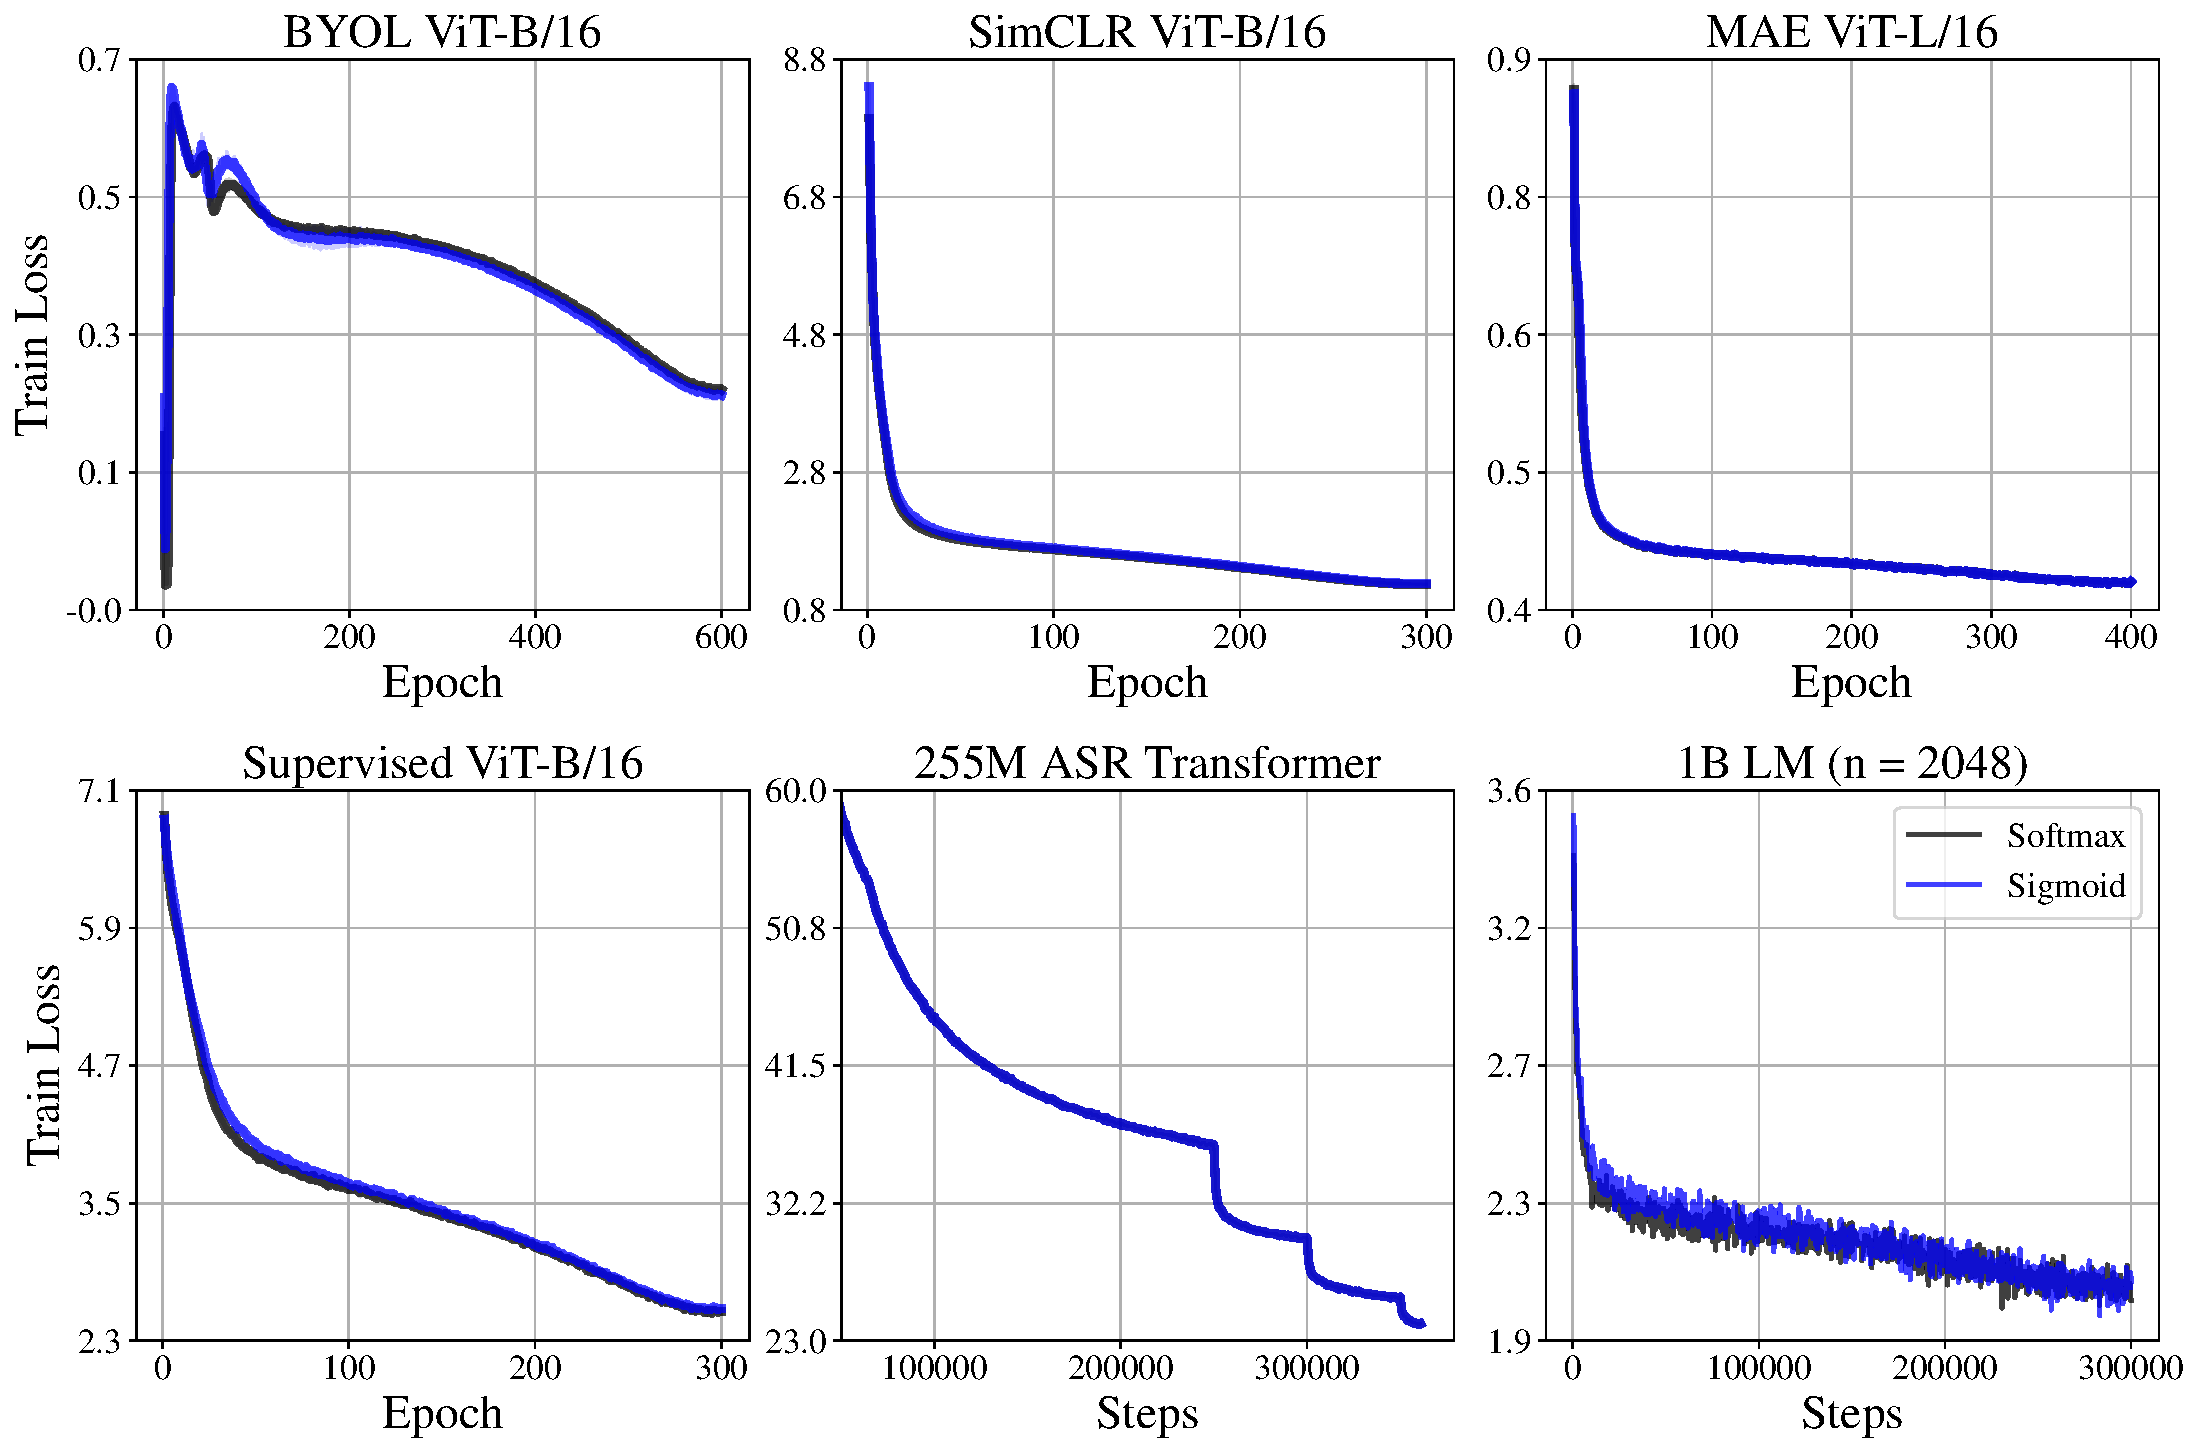
\includegraphics[width=\textwidth]{figures/train_nll_softmax_vs_sigmoid_v4.pdf}
\caption{Train losses comparing $\sigmoidattn$ with $\softmaxattn$.}
\label{fig:summary_nll}
\end{figure}
To empirically validate $\sigmoidattn$, we evaluate across several domains: supervised image classification using vision transformers \citep{DBLP:conf/iclr/DosovitskiyB0WZ21}, self-supervised image representation learning with SimCLR \citep{DBLP:conf/icml/ChenK0H20, DBLP:conf/icml/ZhaiLLBR0GS23}, Bootstrap Your Own Latent (BYOL) \citep{DBLP:conf/nips/GrillSATRBDPGAP20, DBLP:conf/nips/BusbridgeRALDCW23} and Masked AutoEncoders (MAE) \citep{DBLP:conf/cvpr/HeCXLDG22} as well as automatic speech recognition (ASR) \citep{synnaeve2019end,conformer} and auto-regressive language modeling (LM) \citep{DBLP:conf/nips/BrownMRSKDNSSAA20}. We also validate sequence length generalization on TED-LIUM v3~\citep{hernandez2018ted} for ASR and in small scale synthetic experiments in \cref{sec:a_se_pair_repeat_prob}.
Across all these domains and algorithms, we demonstrate that $\sigmoidattn$ matches the performance of $\softmaxattn$ (\cref{fig:summary_nll,fig:test_top1_results}), while offering training and inference speed-ups as highlighted in \cref{sec:FlashSigmoidHardwareAwareImplementation}. Empirically we make the following observations:
\begin{enumerate}[itemsep=0pt,leftmargin=*]
    \item $\sigmoidattn$ is effective for vision tasks without a bias (except MAE), but relies on LayerScale to match the performance of the baseline $\softmaxattn$ (\cref{fig:imagenet_top_1_ablations}-a) in a hyper-parameter free manner.\footnote{\Cref{sec:layerscale_free_sigmoid} demonstrates that supervised vision tasks using $\sigmoidattn$ without LayerScale can match baseline $\softmaxattn$ performance by relying on \emph{learnable} scalar bias and temperature: $\{b, t\} \in \mathbb{R}$.} All results presented for $\softmaxattn$ also fairly add LayerScale unless specified.
    \item LM and ASR are sensitive to the initial norm $|| \sigma(\mQ \mK^T/\sqrt{d_{qk}}) \mV ||$. Modulation is required via (a) relative positional embeddings like ALiBi \citep{DBLP:conf/iclr/PressSL22}, which reduces the initial attention norm by shifting logit mass to the zero regime under $\sigmoidattn$, (b) appropriate initialization of $b$ to achieve the same effect -- enabling usage of any positional embedding.
\end{enumerate}

\begin{figure}[htbp]
    \centering
    \begin{minipage}{0.48\textwidth}
        \centering
        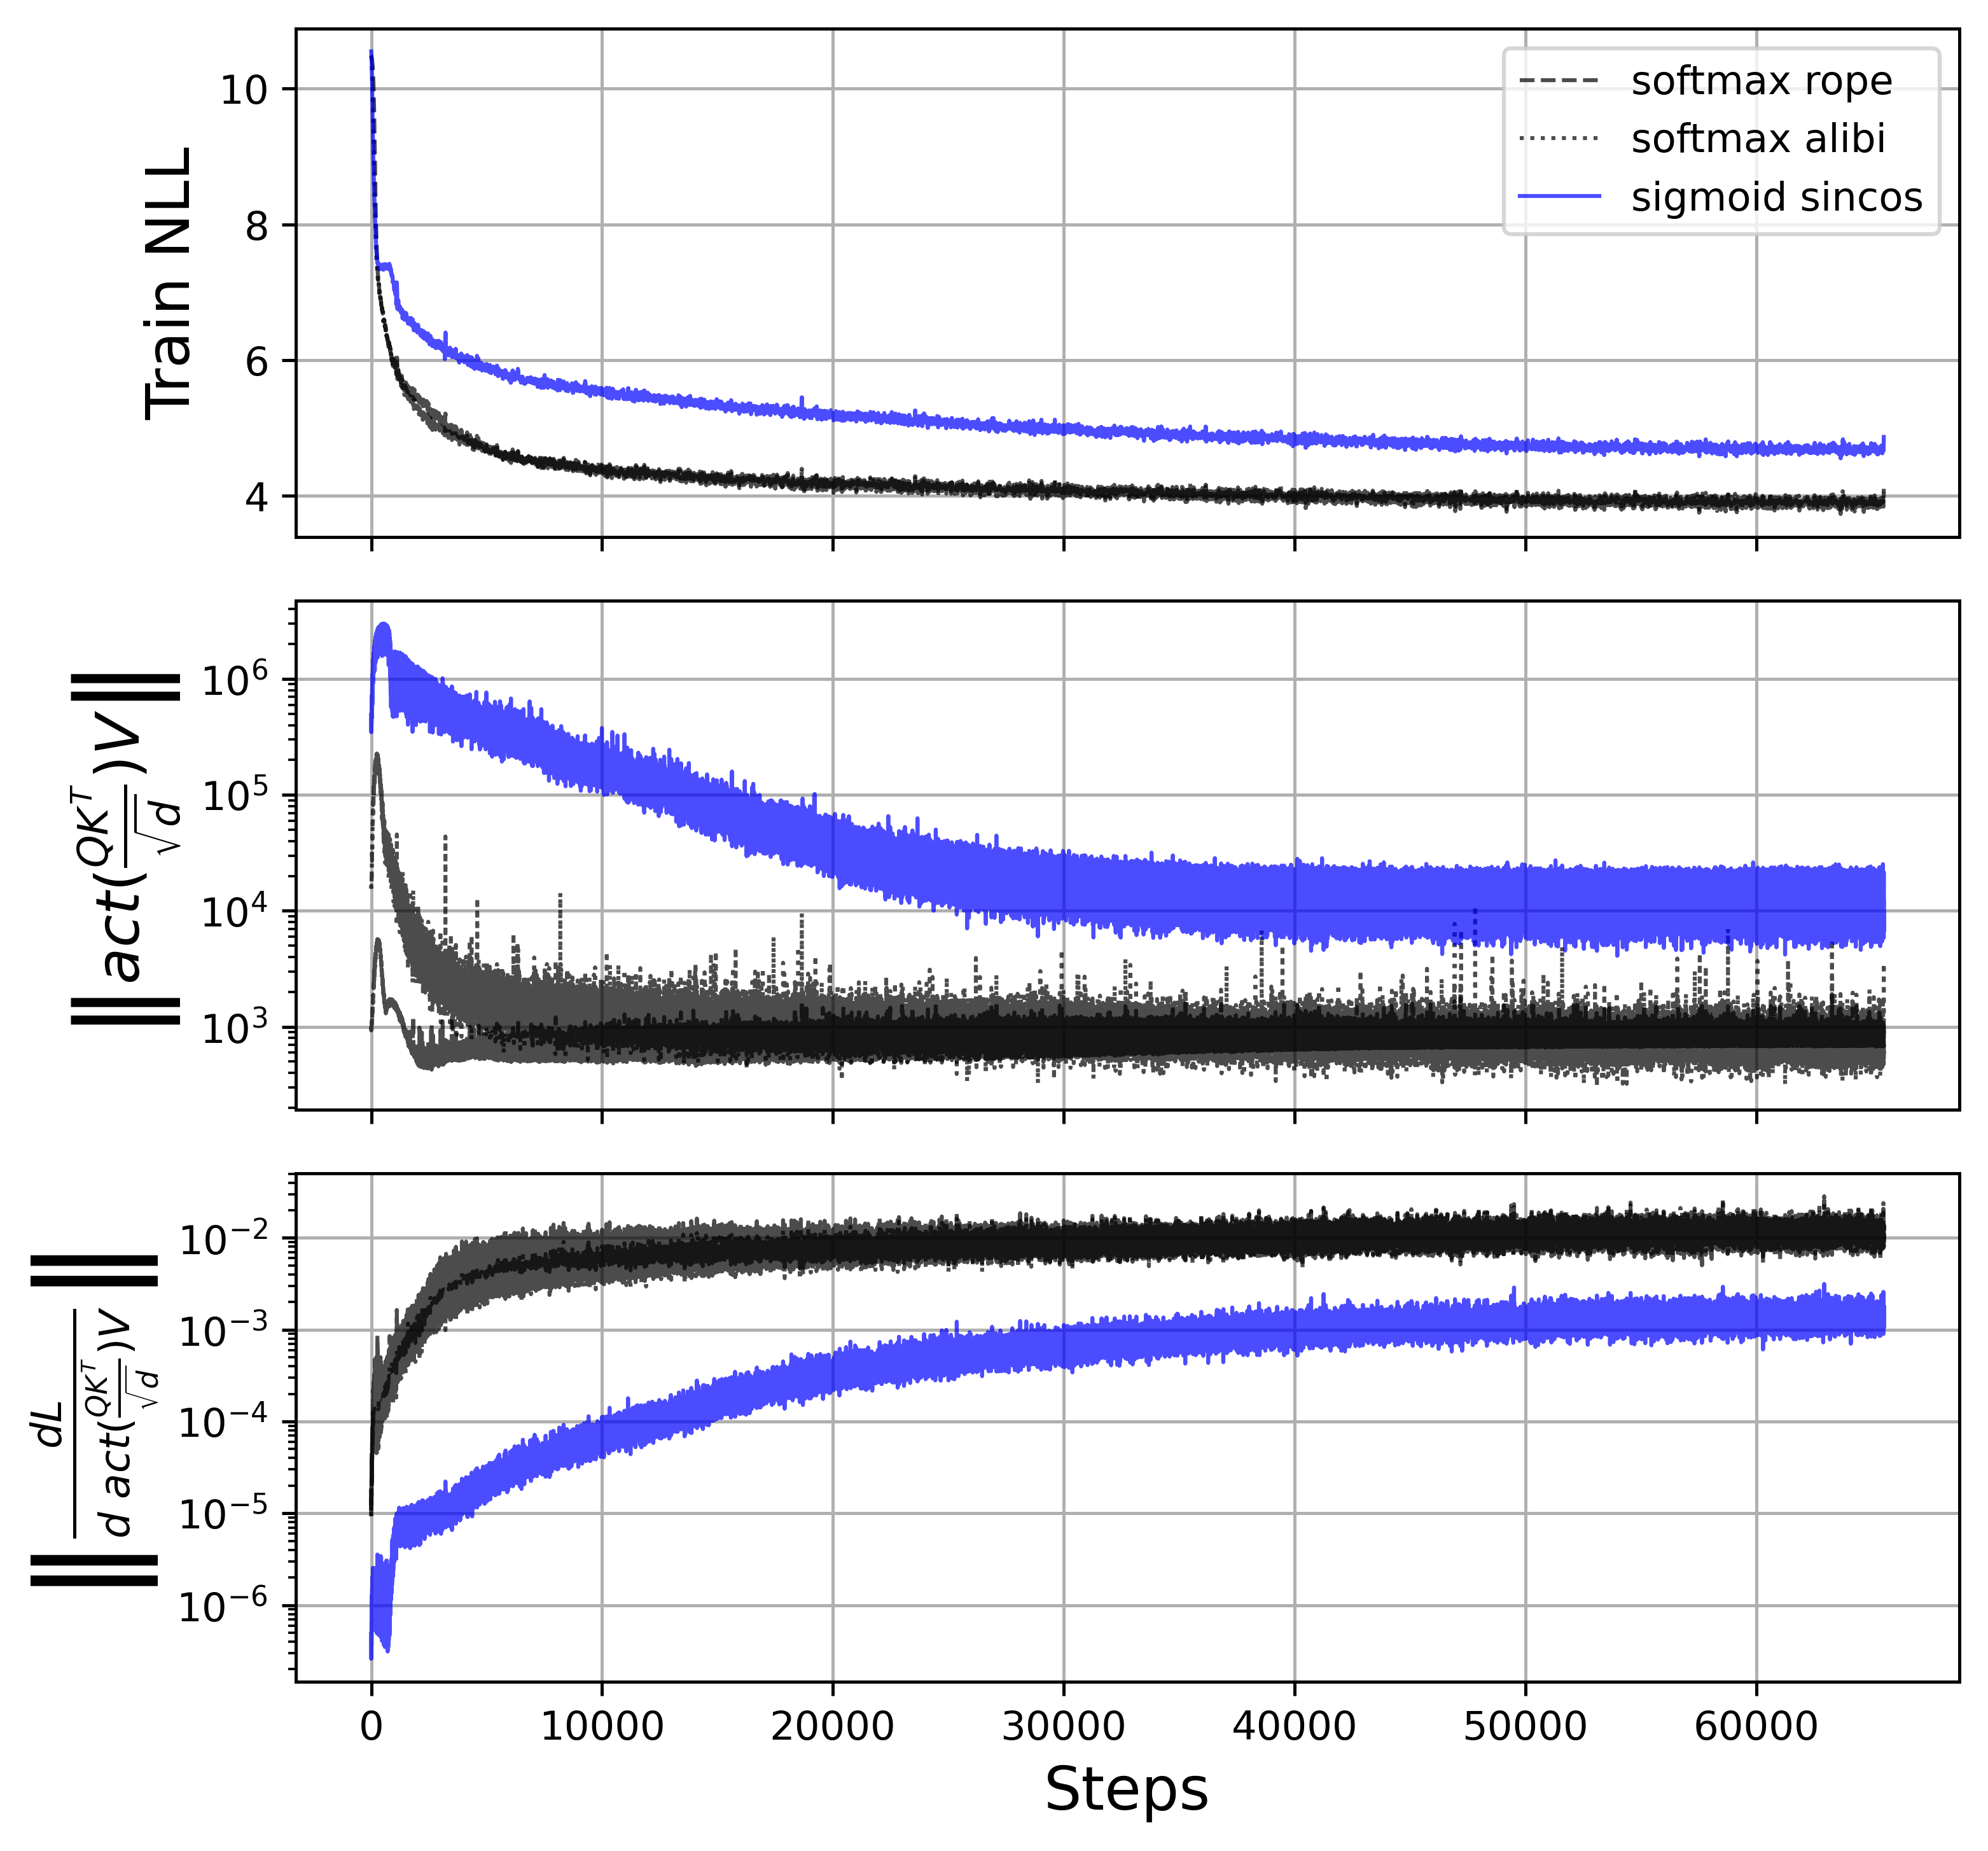
\includegraphics[width=\textwidth]{figures/attn_norm_seed1000001_softmax_rope_vs_softmax_alibi_vs_sigmoid_sincos.png}    
        \captionsetup{justification=centering}
        \caption{$\sigmoidattn$ with SinCos.}
        \label{fig:rope_vs_sincos}
    \end{minipage}\hfill
    \begin{minipage}{0.48\textwidth}
        \centering        
        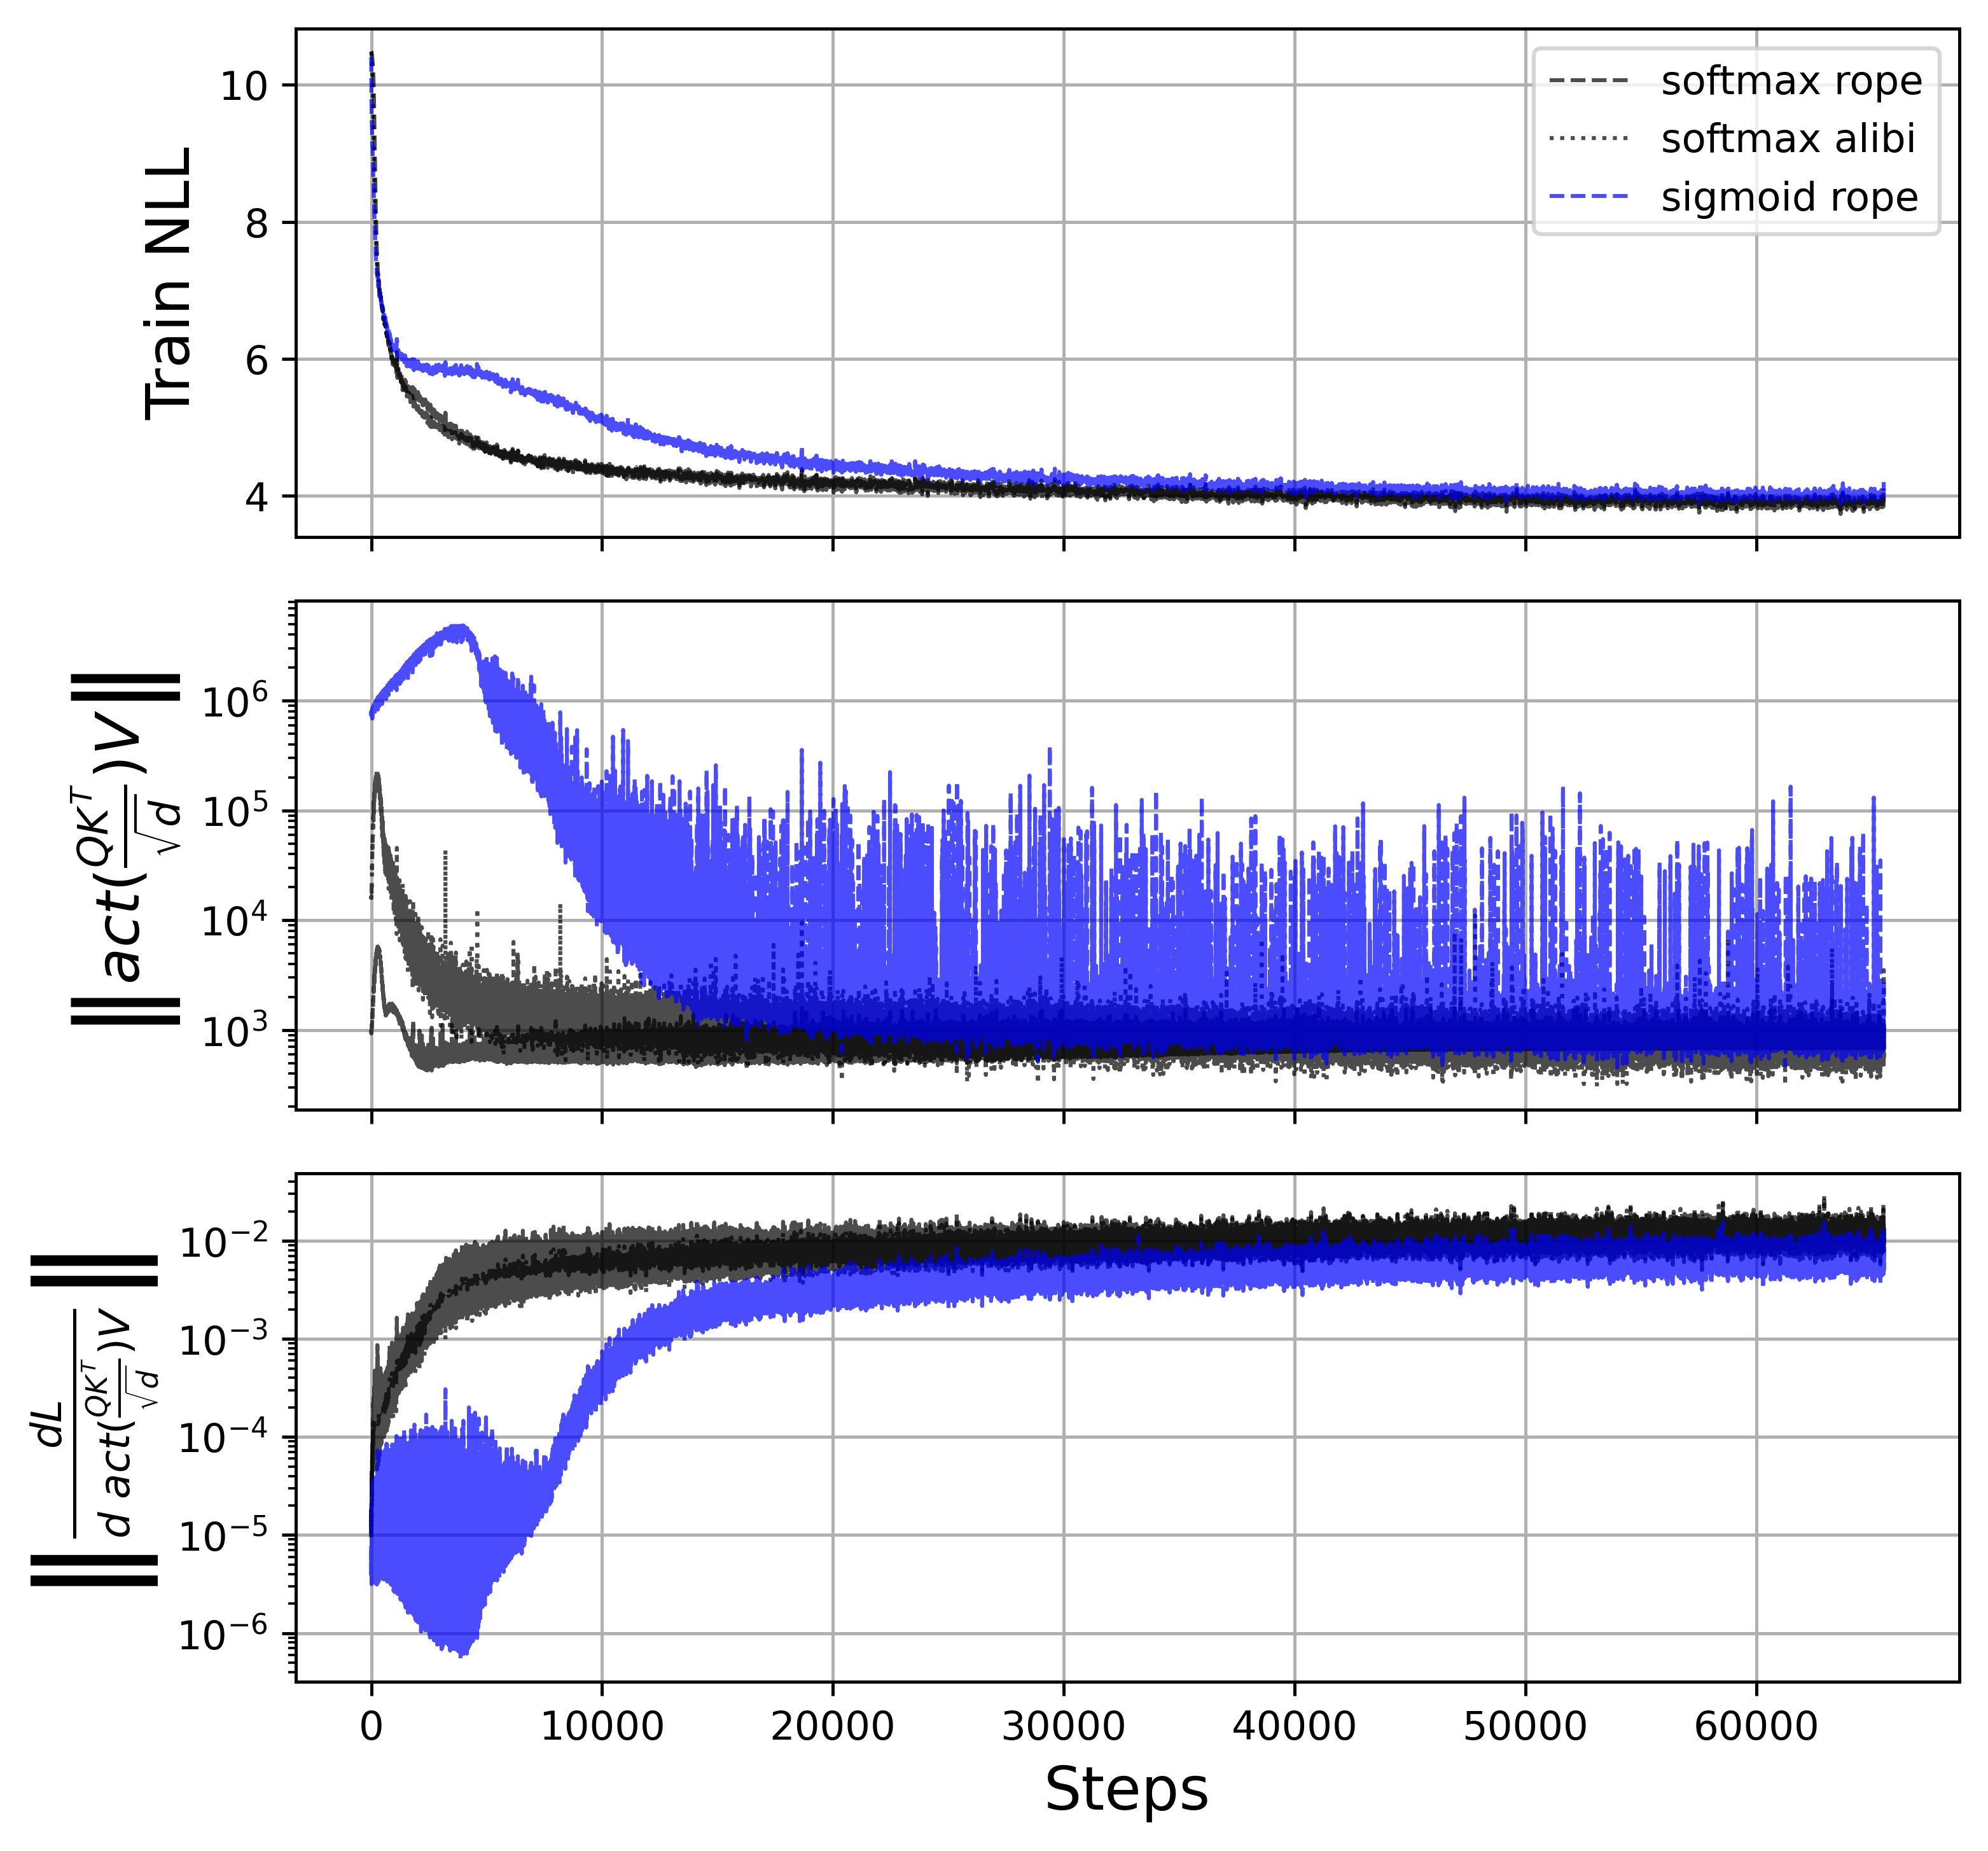
\includegraphics[width=\textwidth]{figures/attn_norm_seed1000001_softmax_rope_vs_softmax_alibi_vs_sigmoid_rope.png}
        \captionsetup{justification=centering}
        \caption{$\sigmoidattn$ with RoPE.}
        \label{fig:rope_vs_rope}
    \end{minipage}
    \hfill
    \begin{minipage}{0.48\textwidth}
        \centering
        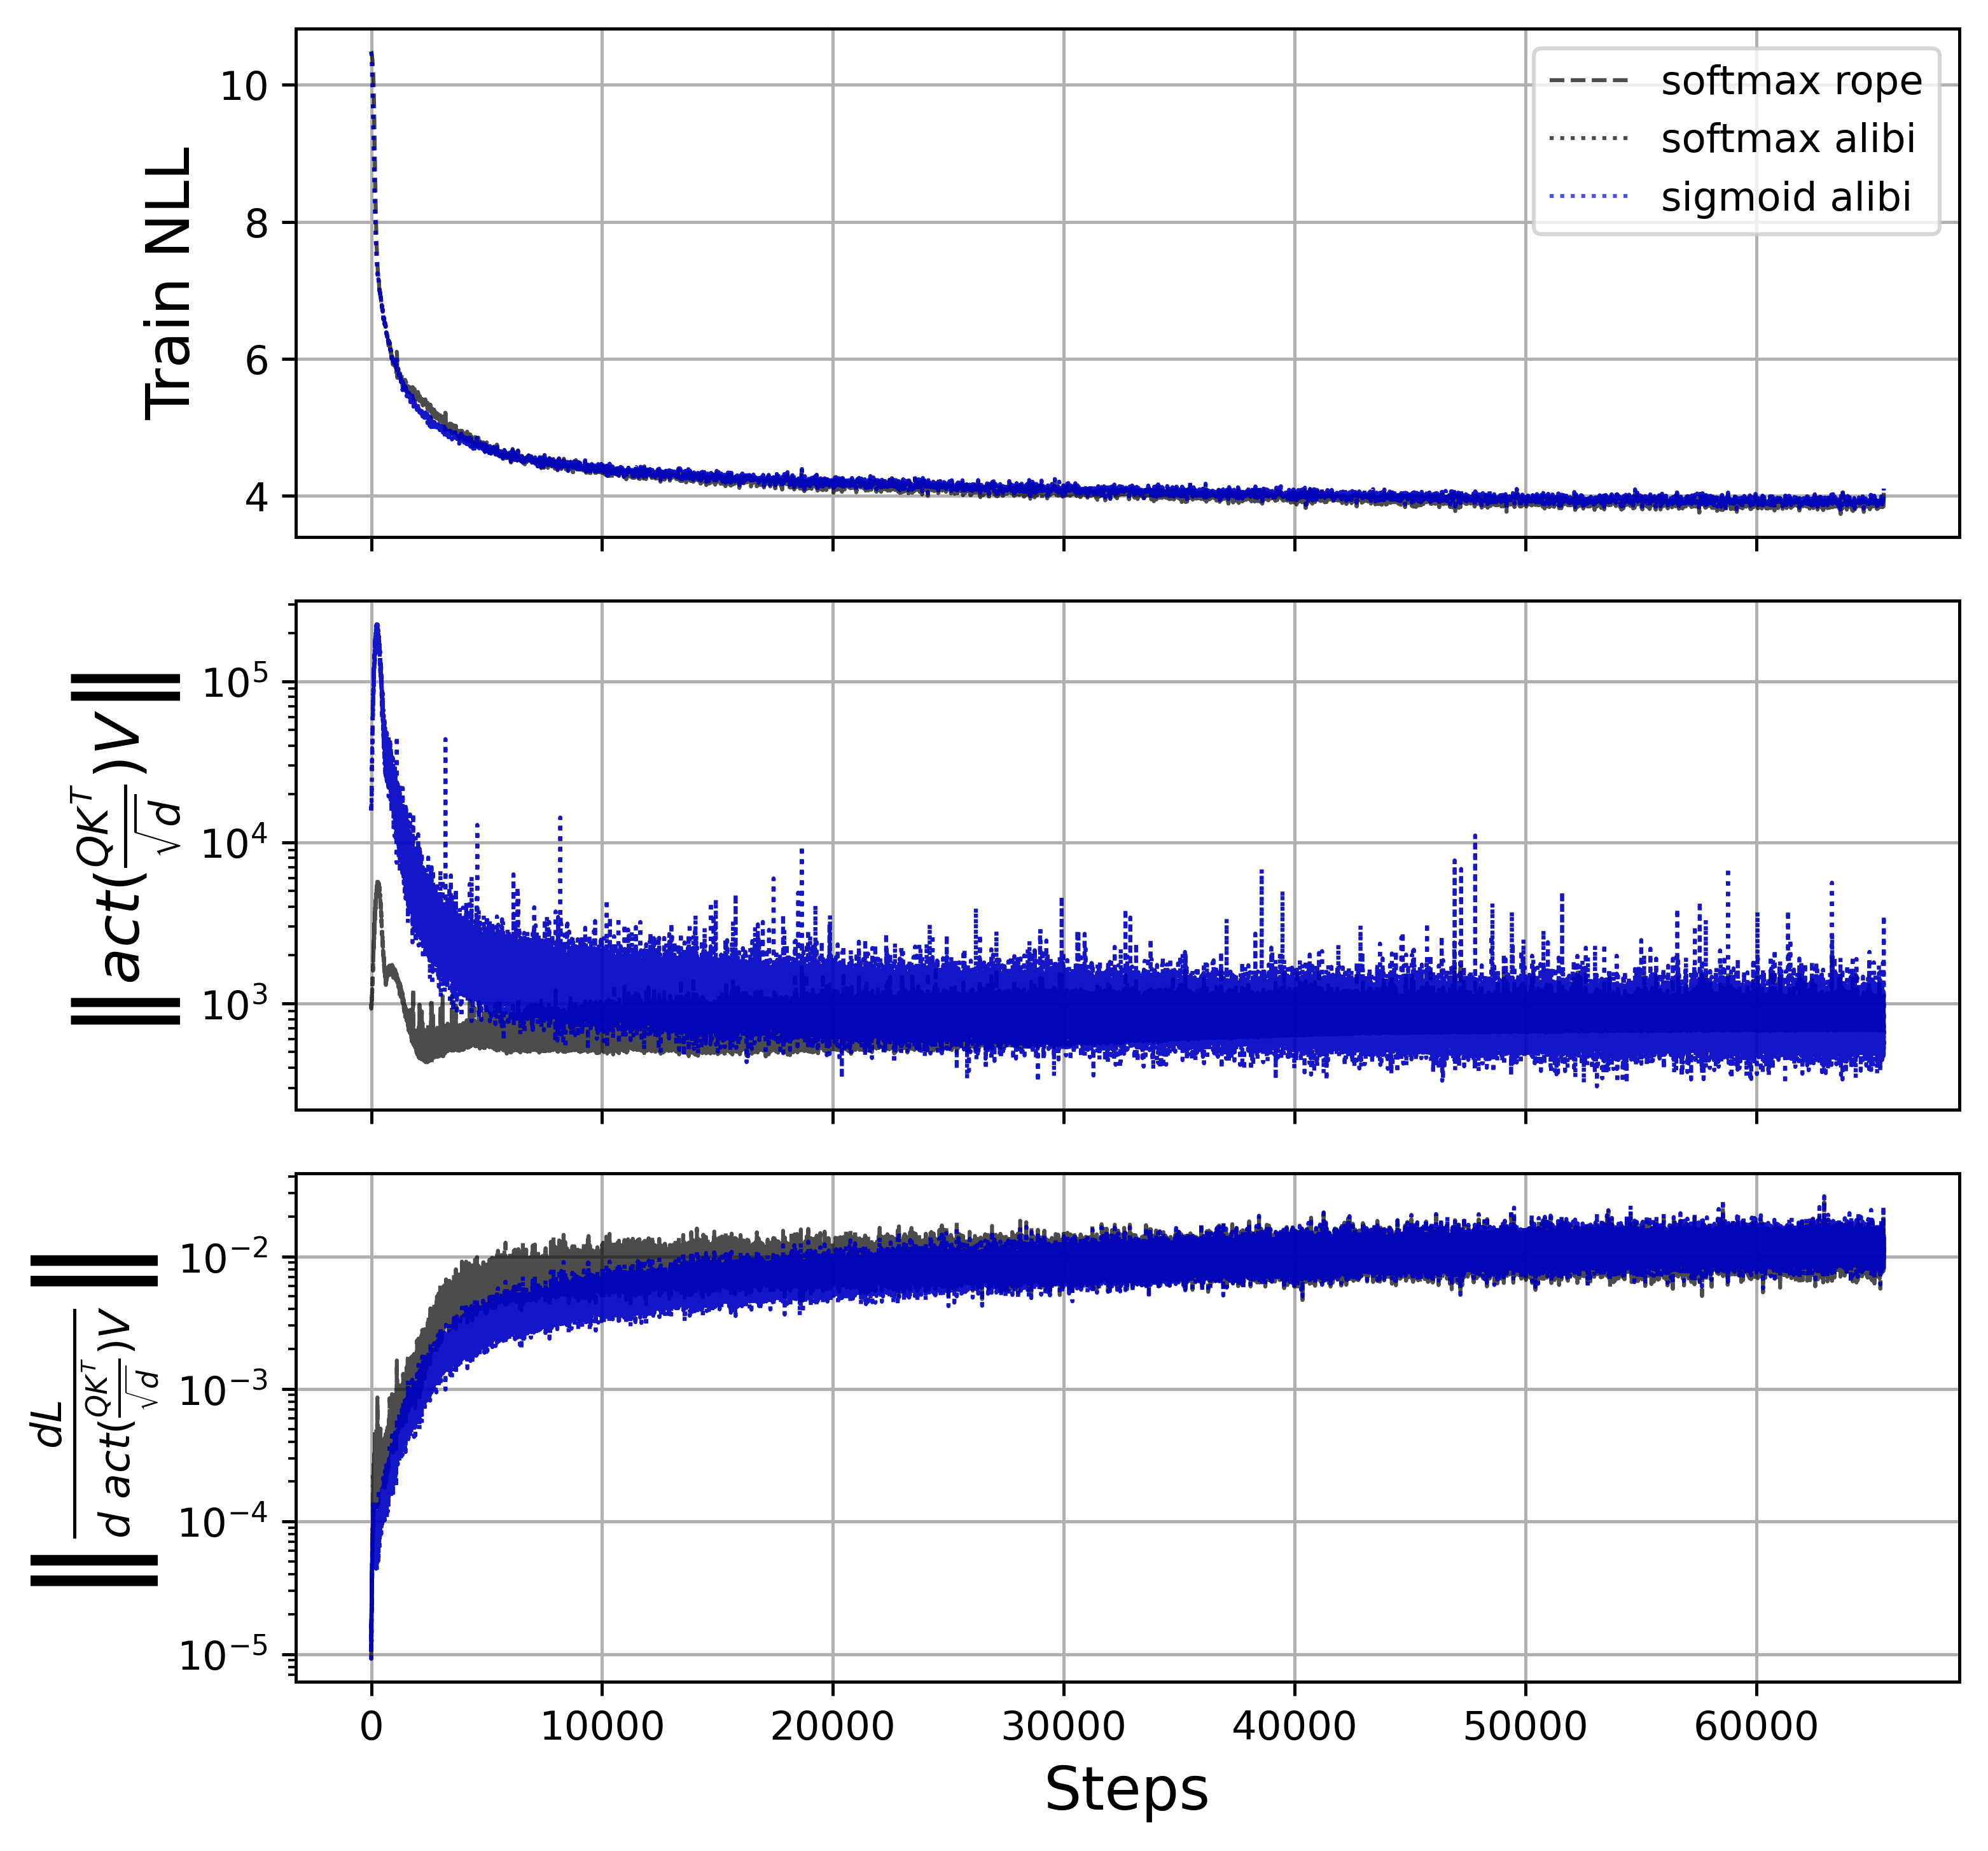
\includegraphics[width=\textwidth]{figures/attn_norm_seed1000001_softmax_rope_vs_softmax_alibi_vs_sigmoid_alibi.png}
        \captionsetup{justification=centering}
        \caption{$\sigmoidattn$ with ALiBi.}
        \label{fig:rope_vs_alibi}
    \end{minipage}\hfill
    \begin{minipage}{0.48\textwidth}
        \centering        
        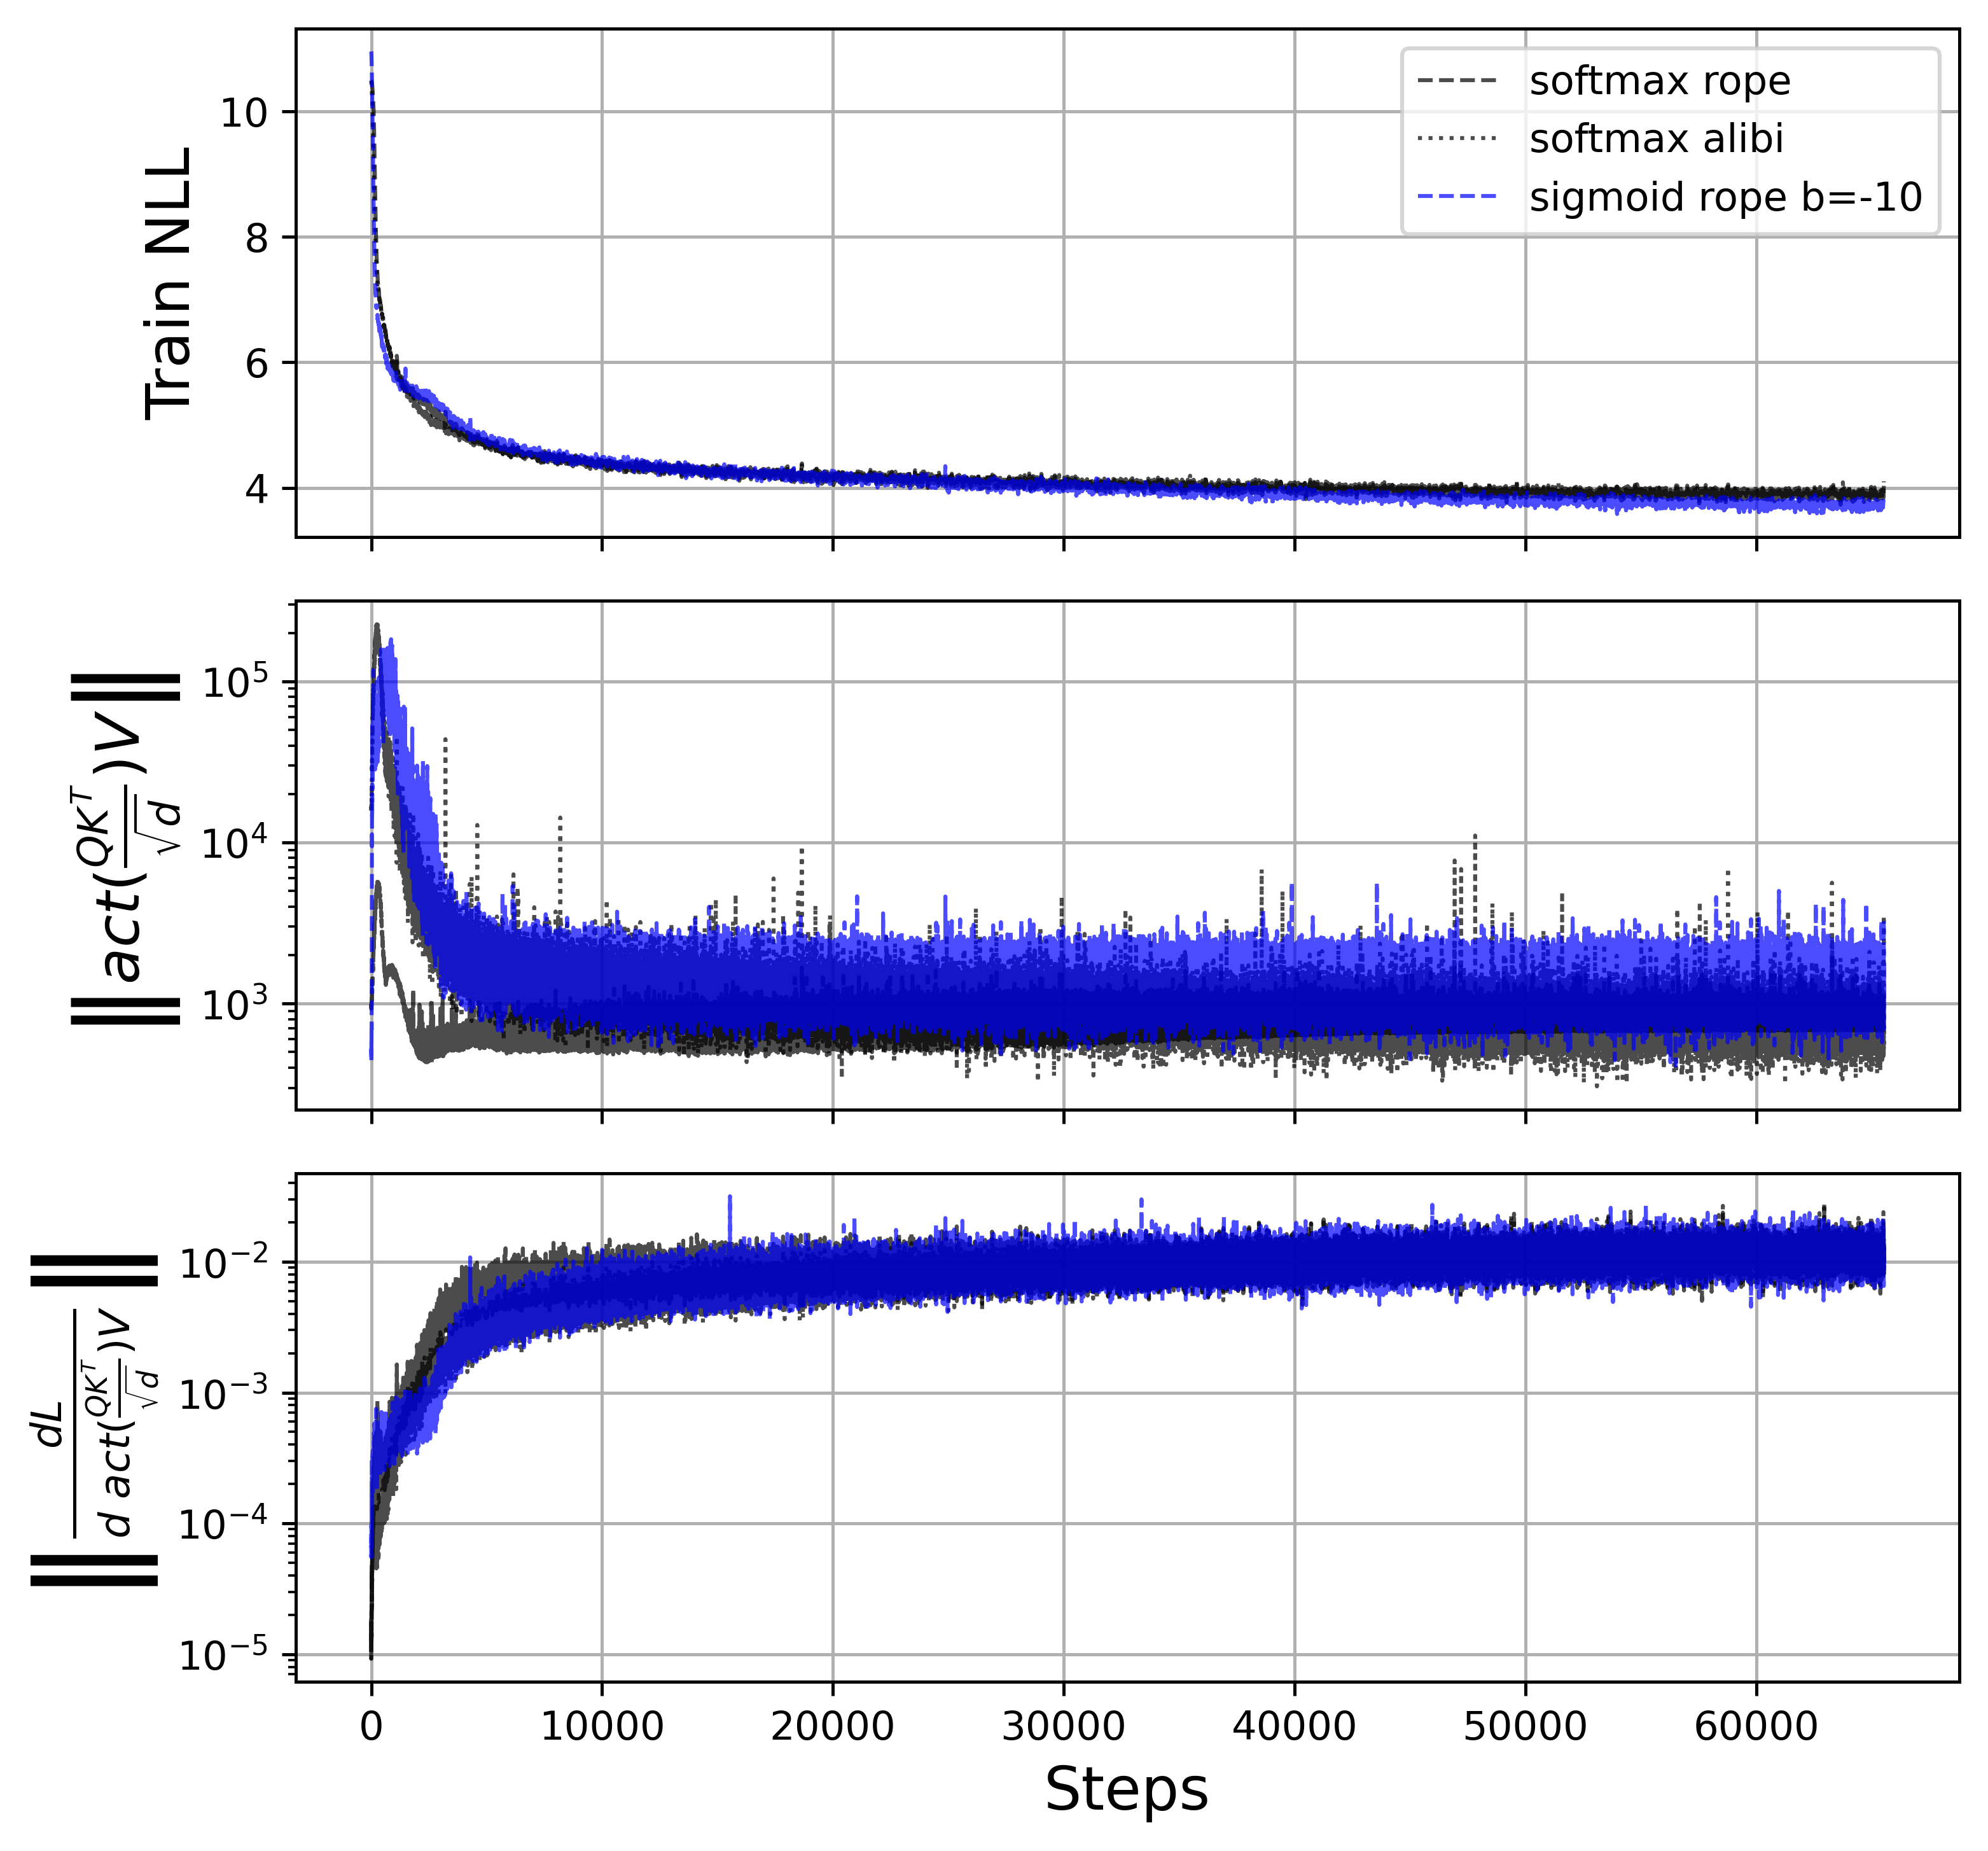
\includegraphics[width=\textwidth]{figures/attn_norm_seed1000001_softmax_rope_vs_softmax_alibi_vs_sigmoid_rope_b=-10.png}
        \captionsetup{justification=centering}
        \caption{$\sigmoidattn$ with RoPE, $b=-10$.}
        \label{fig:rope_vs_rope_b-10}
    \end{minipage}  
    \vspace{-0.4cm}
\end{figure}

\subsection{Ablations}
\label{sec:ablations}
We begin with ablations to dissect the benefits of each of our introduced components. To gain intuition about $\sigmoidattn$, we developed a research-friendly auto-regressive (AR) LM training framework to measure all components of attention and validate the effects of LayerScale, LayerNorm applied to Q and K (QK norm), different positional embedding techniques, and initialization values for $b$.
\begin{figure}[h]
    \centering
    \begin{minipage}[t]{0.48\textwidth}
        \centering
        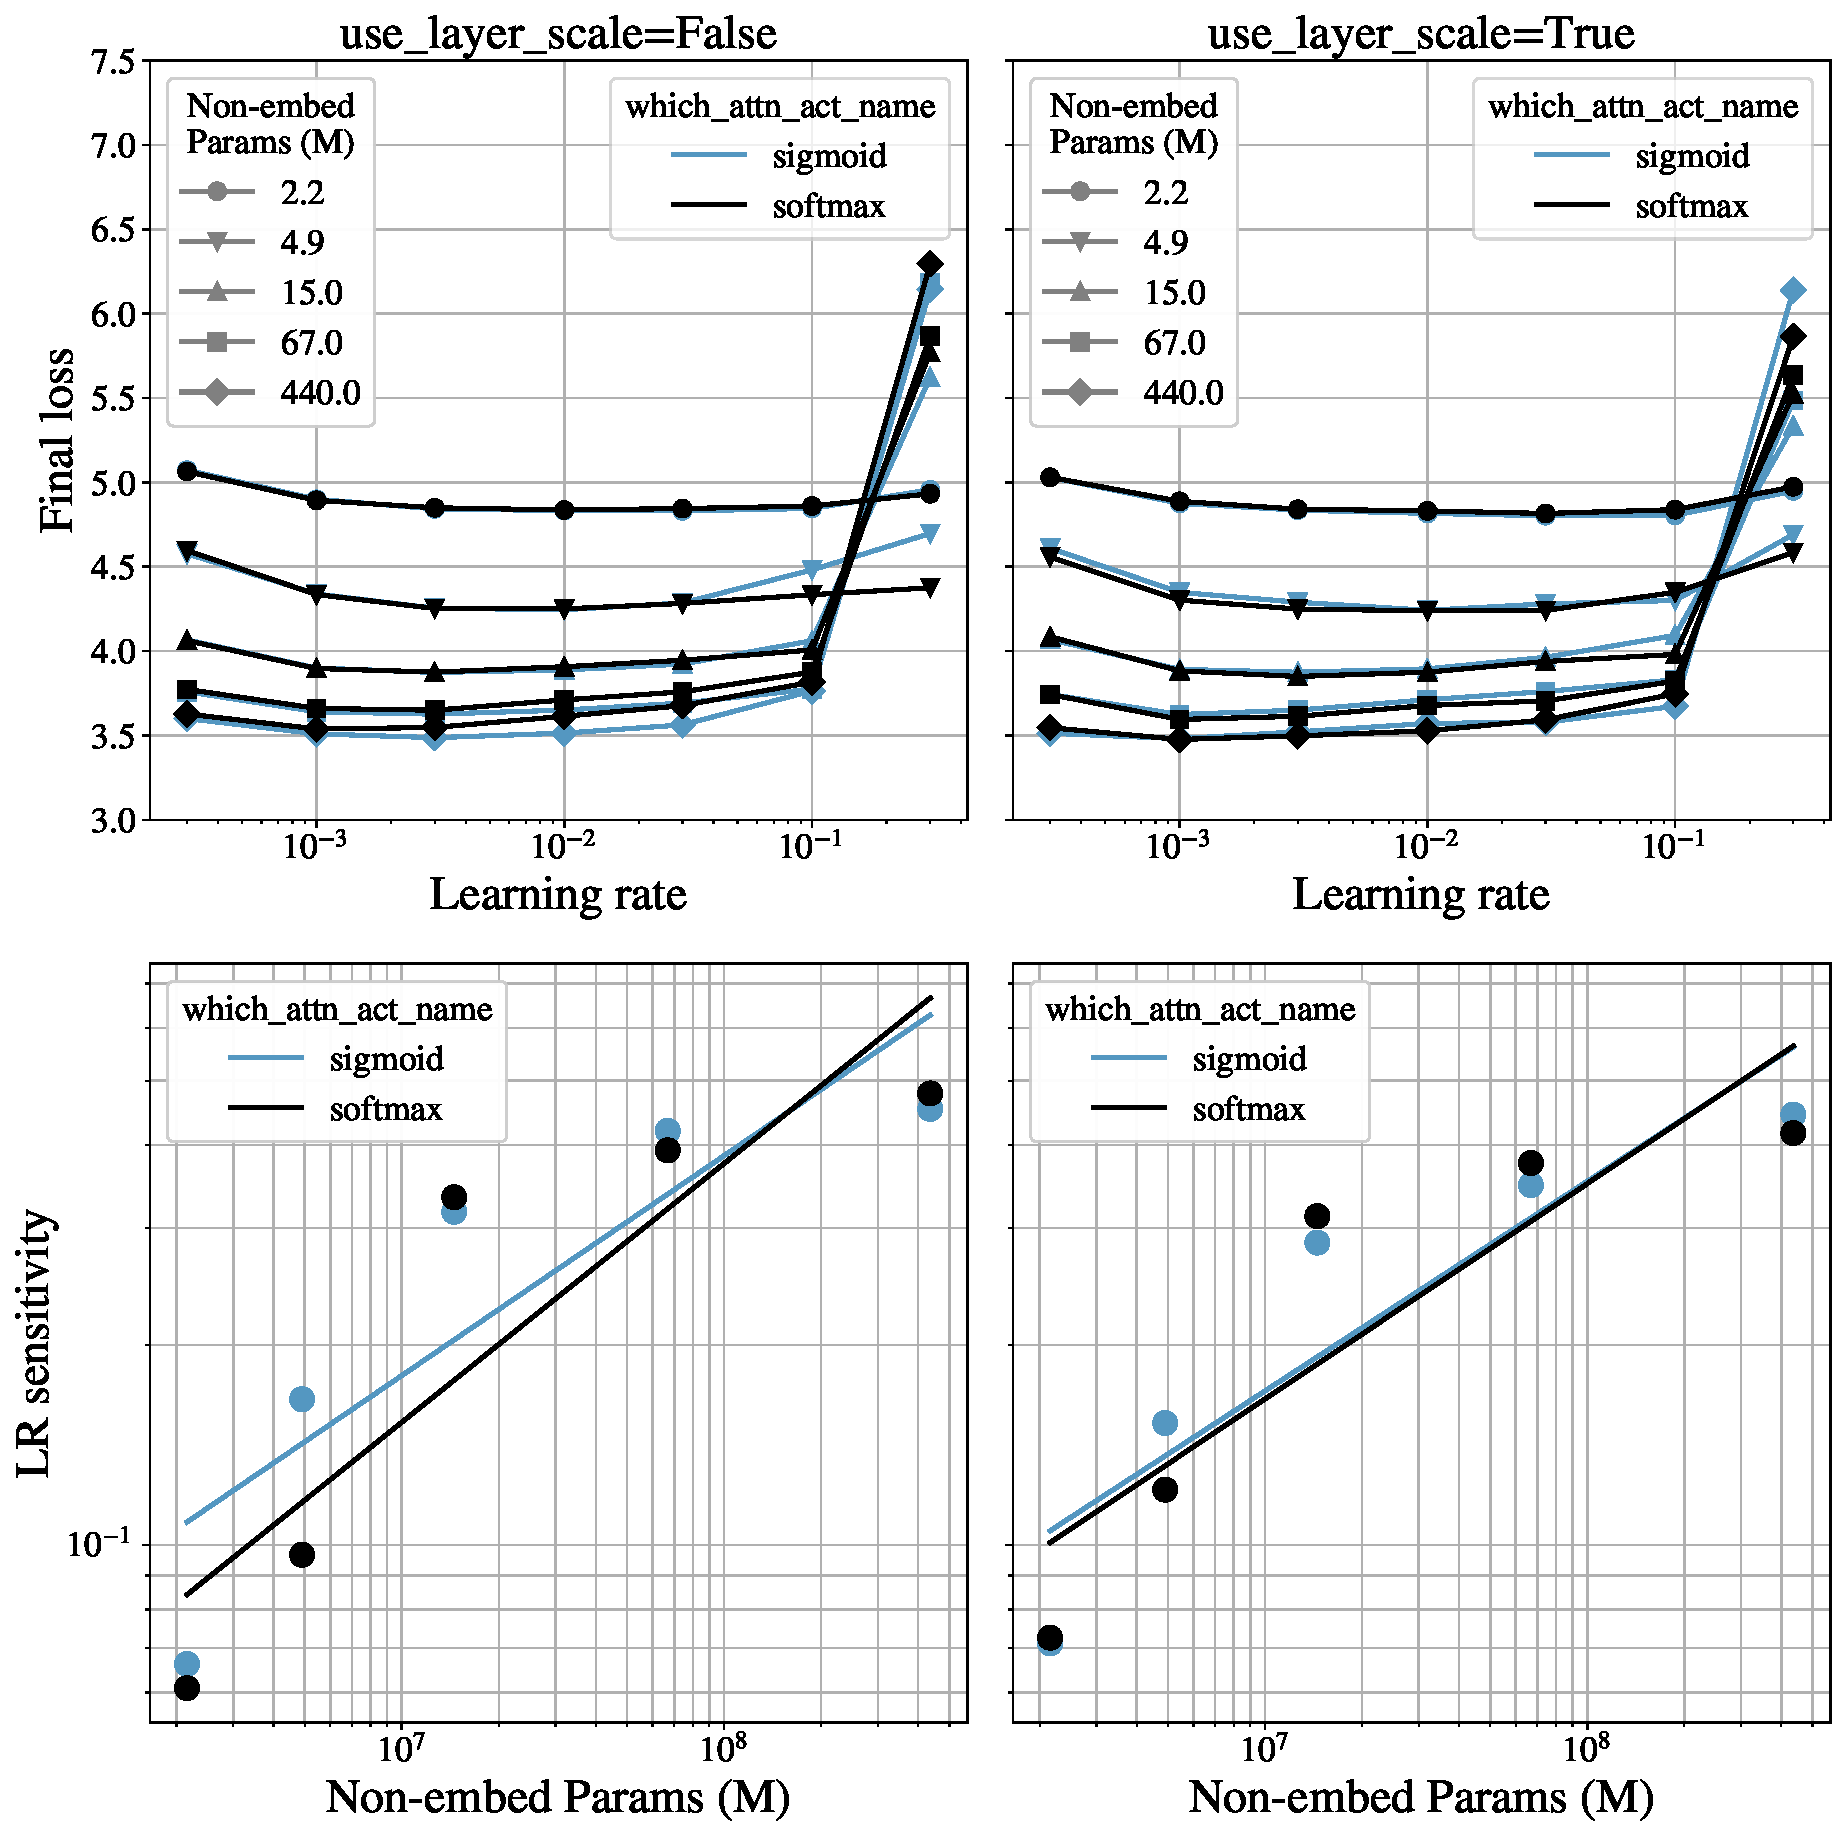
\includegraphics[width=\textwidth]{figures/lines=activation-cols=layerscale_with_log_n_or_max3std.pdf} 
        \caption{LR sensitivity LayerScale ablation.}
        \label{fig:layerscale_ablation}
    \end{minipage}%
    \hfill
    \begin{minipage}[t]{0.48\textwidth}
        \centering
        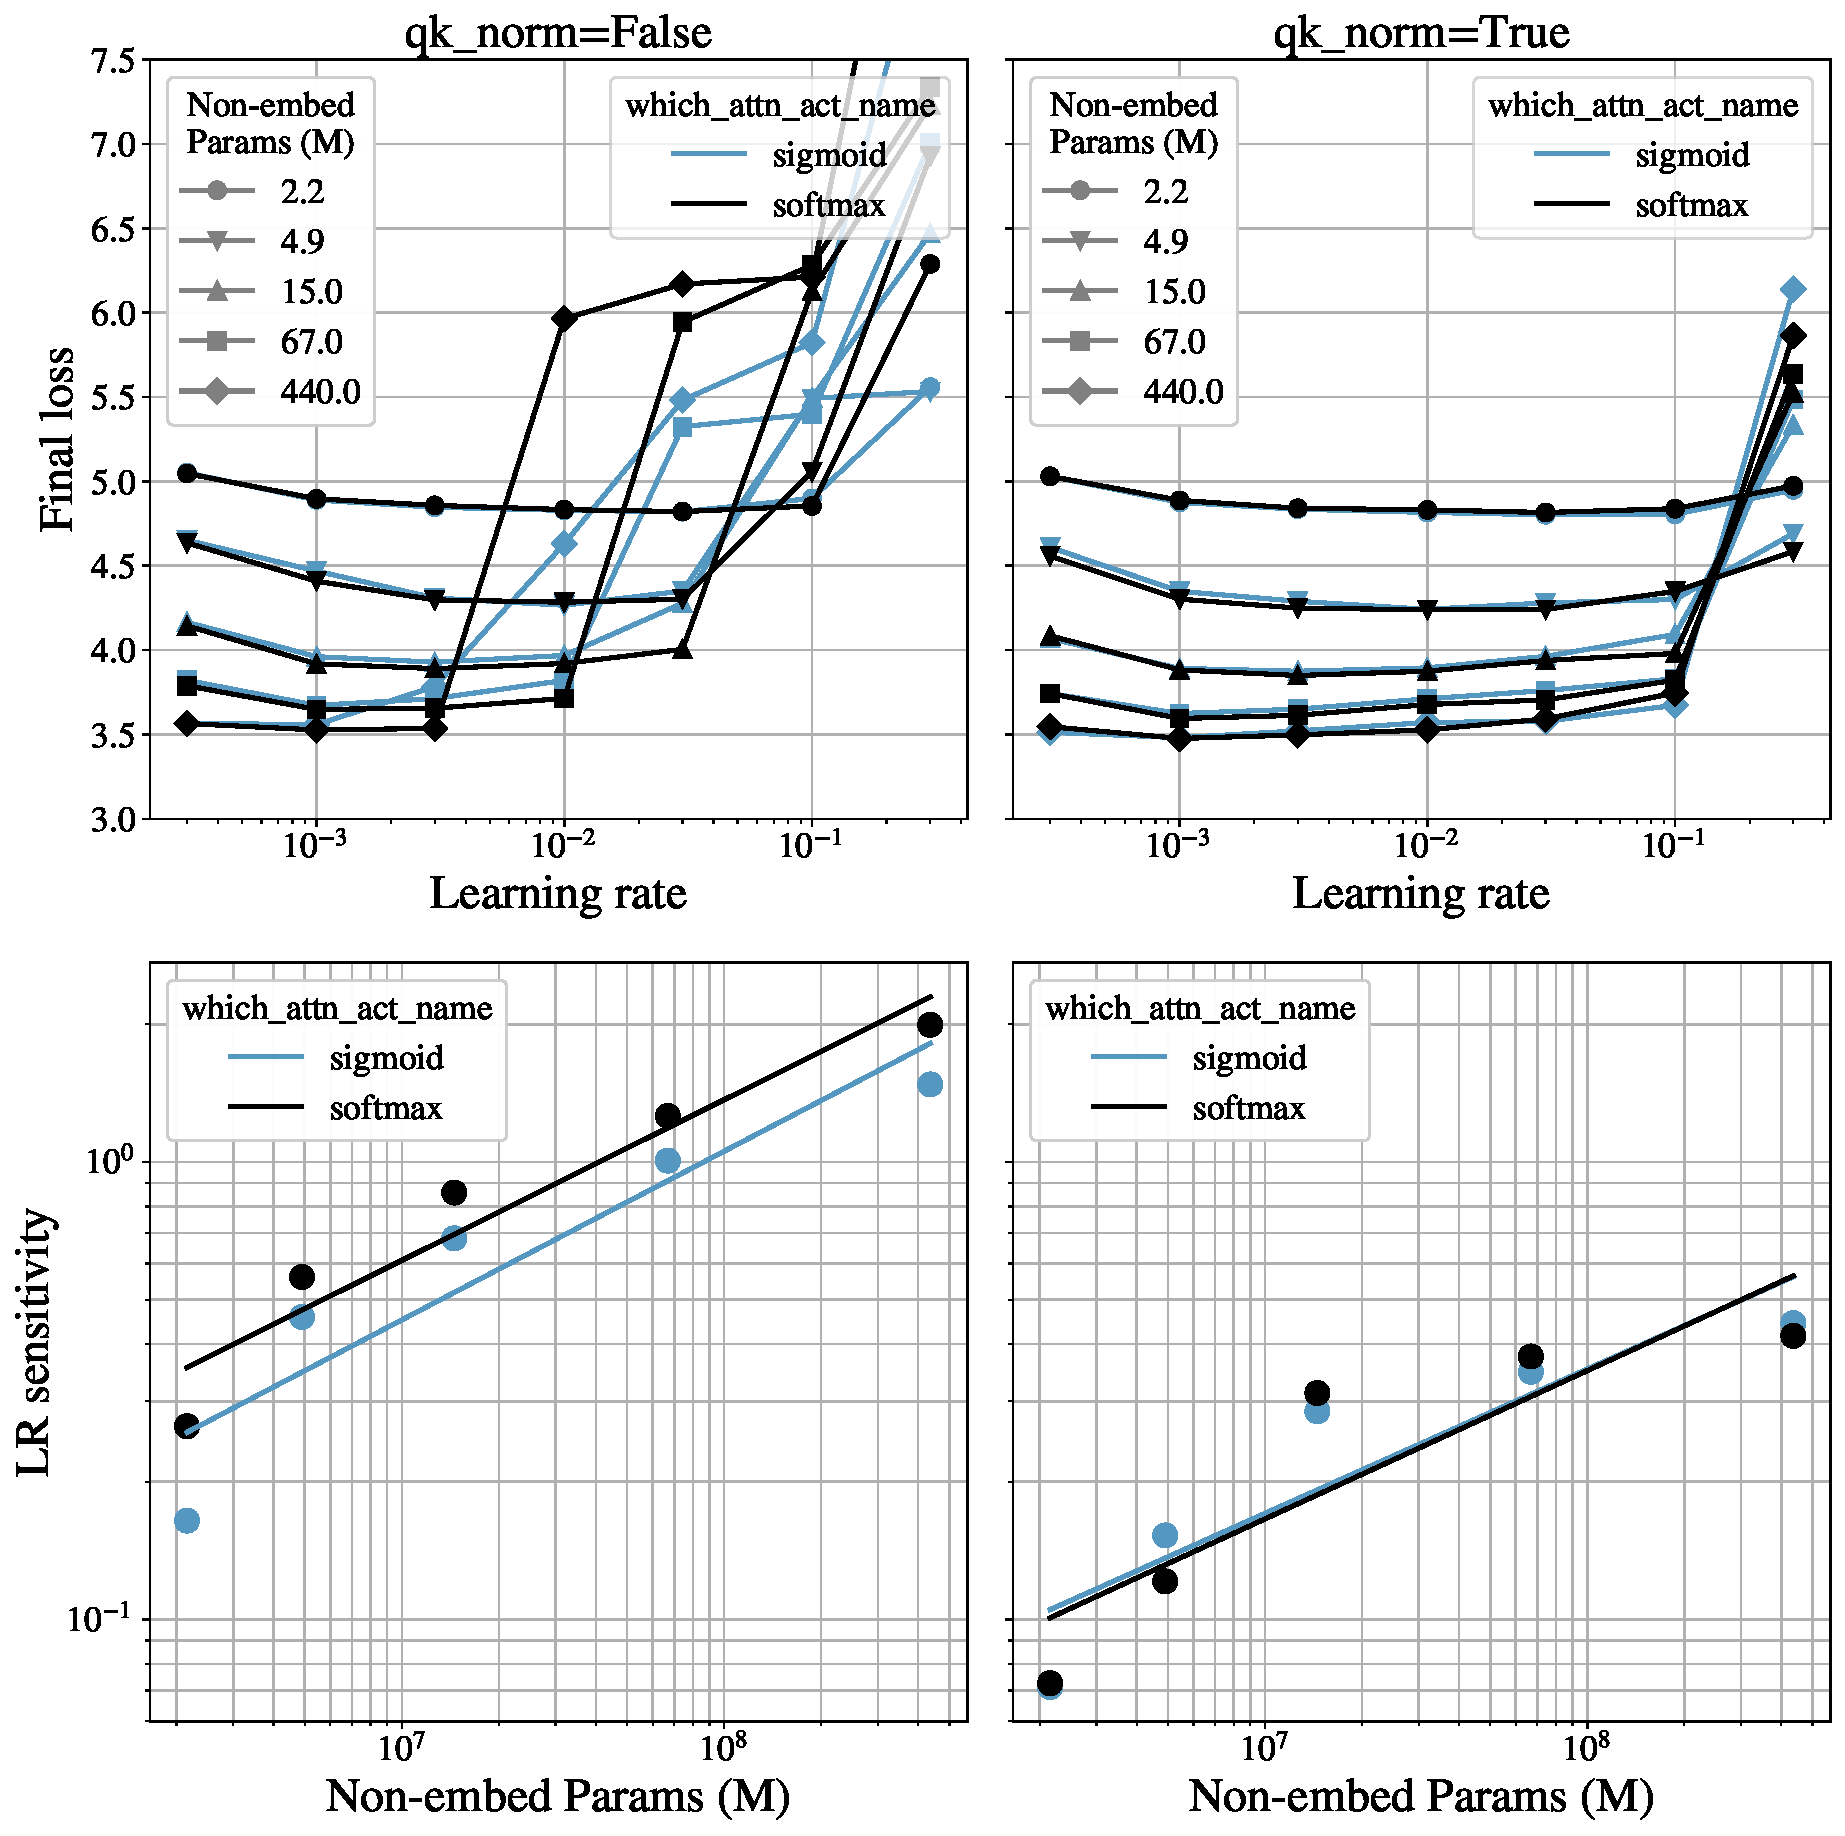
\includegraphics[width=\textwidth]{figures/lines=activation-cols=qknorm_with_log_n_or_max3std.pdf}
        \caption{LR sensitivity QK norm ablation.}
        \label{fig:qk_norm_ablation}
    \end{minipage}
\end{figure}
\begin{figure}[h]
    \centering
    \vspace{-0.2cm}
    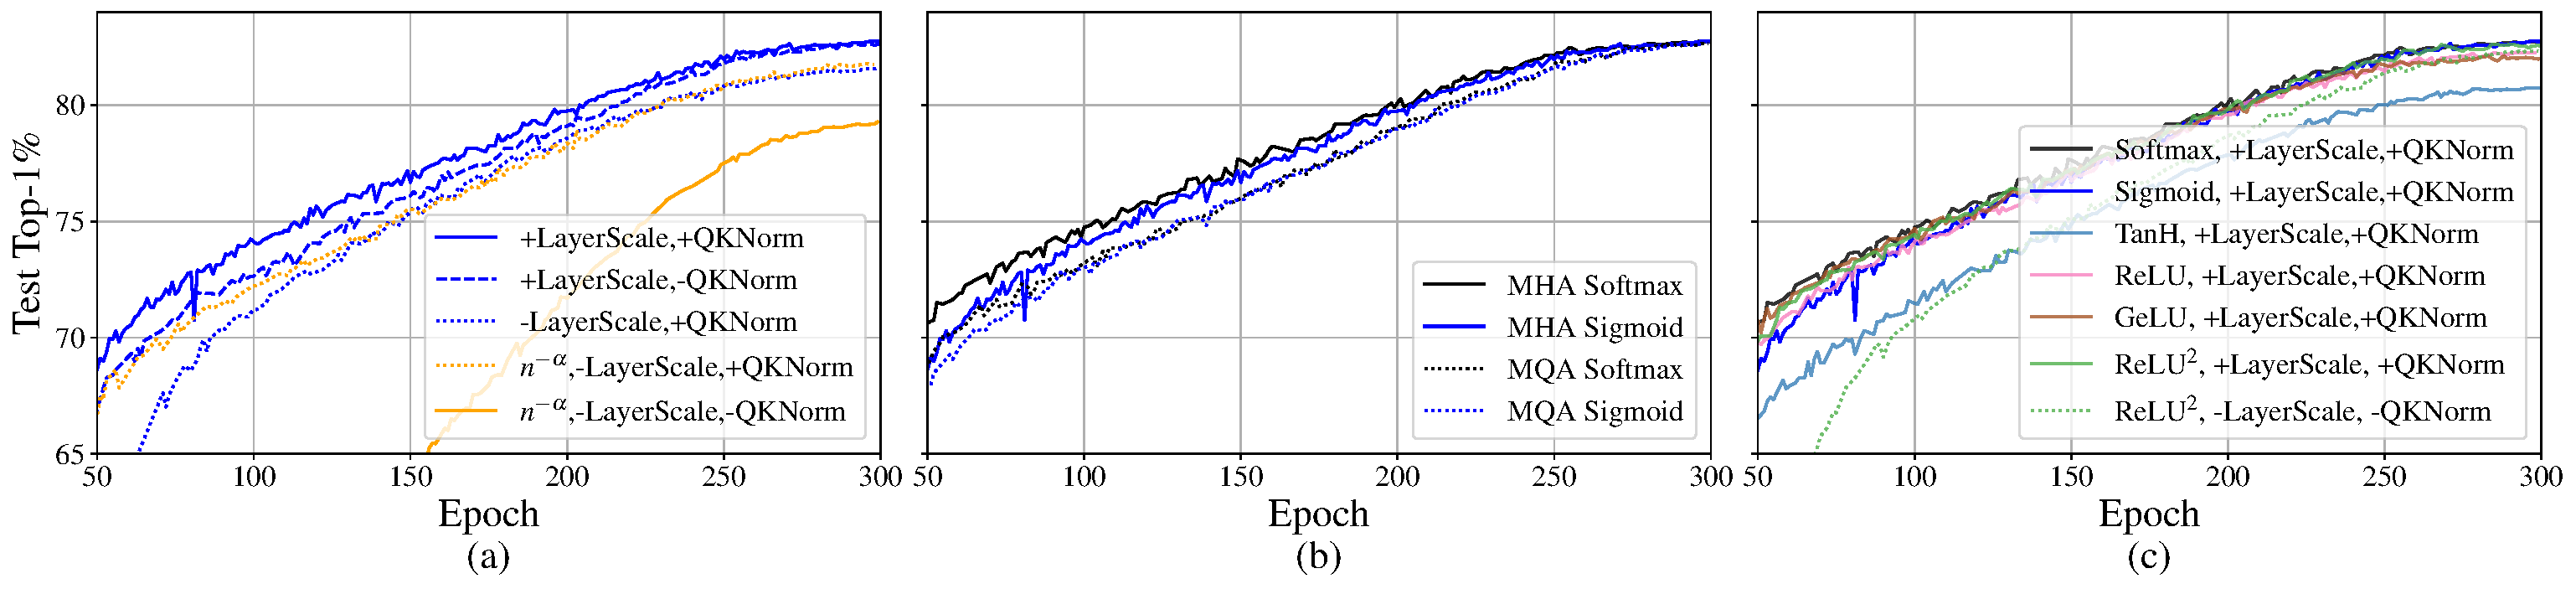
\includegraphics[width=\textwidth]{figures/imagenet_ablations_top1.pdf}
    \caption{ImageNet1k ViT-B/16 classification. (a) $\sigmoidattn$ is robust without QK norm (+LayerScale, -QKNorm). Removing LayerScale reduces accuracy by 1.0\% (-LayerScale, +/-QKNorm). $n^{-\alpha}$ normalization \citep{wortsman2023replacing} underperforms without LayerScale. (b) $\sigmoidattn$ multi-query attention (MQA) \citep{DBLP:journals/corr/abs-1911-02150} with one head matches multi-head attention (MHA). (c) Sigmoid with LayerScale and QK norm performs comparably to other activations, except TanH. ReLU$^2$ \citep{DBLP:conf/icml/HuaDLL22} underperforms without LayerScale and QK norm.}
    \label{fig:imagenet_top_1_ablations}
    \vspace{-0.4cm}
\end{figure}
\paragraph{Mitigating Large Attention Norms} We train a single layer AR transformer block (E=3072, D\_FF=12288) on the realnews split of C4 \citep{DBLP:journals/jmlr/RaffelSRLNMZLL20}. We train for $2^{16}$ steps using a batch size of 6 and max sequence length of 4096 using a single cycle cosine learning rate (LR) schedule without weight decay. $\sigmoidattn$ initially underperformed $\softmaxattn$ when using absolute sinusoidal (SinCos) (\cref{fig:rope_vs_sincos}) or relative (\cref{fig:rope_vs_rope}) positional embeddings (PE), which we attribute to high initial attention Frobenius norms, $\lVert \sigma(\mQ \mK^T / \sqrt{d}) \mV \rVert$. A corresponding evolution of the attention distribution and sparsity can be seen in Appendix \cref{fig:attn_evolve} and \cref{fig:attn_metric_evolve} on a synthetic task.
To address these larger attention norms, we propose: (a) using ALiBi \citep{DBLP:conf/iclr/PressSL22} whose relative bias moves initial attention logit mass to the zero region under the sigmoid activation, producing equivalent train negative log-likelihoods (\cref{fig:rope_vs_alibi}); or (b) set the attention logit bias $b$ to a negative offset proportional to the sequence length, $b \propto -\ln n$ (see \cref{sec:attn_bias_ablation} for an ablation on $b$). This enables the usage of other PE techniques like RoPE~\citep{DBLP:journals/ijon/SuALPBL24} (\cref{fig:rope_vs_rope_b-10}). 
\paragraph{LayerScale} To validate the need for LayerScale, we follow \citet{DBLP:journals/corr/abs-2309-14322} to quantify the impact on stability.
All models are trained with RoPE with $b \propto -\ln n$, using AdamW  \citep{loshchilov2017decoupled} on the 
realnews split of C4 
with $(\beta_1,\beta_2)=(0.9, 0.95)$, $\eps=10^{-8}$,  $wd=0$, 
batch size 24, maximum token sequence length of 512 from the T5 tokenizer \citep{DBLP:journals/jmlr/RaffelSRLNMZLL20}, cosine LR schedule of $2^{14}$ steps including a linear warmup of $2^{10}$ steps. 
Models have 
$n_{\text{heads}}=\kappa$,
$n_{\text{layers}}=2\times \kappa$,
$d_{\text{model}}=64\times \kappa$ and
$d_{\text{feed-forward}}=256\times\kappa$
for a scaling value $\kappa\in\{1,2,4,8,16\}$
leading to models with $\{2.2, 4.9,15.0,67.0,440.0\}M$ trainable non-embedding parameters.
Following \citet{DBLP:journals/corr/abs-2309-14322},
we sweep learning rates
$\eta\in \{3\times 10^{-4}, 1\times 10^{-3}, 3\times 10^{-3}, 1\times 10^{-2}, 3\times 10^{-2}, 1\times 10^{-1}, 3\times 10^{-1}\}$.
LR sensitivity is defined as 
$\mathbb E_{\eta\in[a,b]}\left[\min(\ell(\mathcal A(\eta)),\ell_0)-\ell^*\right]$
where $\ell(\mathcal A(\eta))$ is the loss achieved by the learning algorithm $\mathcal A$ with LR $\eta$,
$\ell_0$ is the loss at initialization, and
$\ell^*$ is the loss achieved by the best LR.
LayerScale is initialized at $10^{-4}$. 
Unlike vision tasks, where LayerScale \emph{improves performance} (\cref{fig:imagenet_top_1_ablations}-a), in LM, we observe that $\softmaxattn$ slightly benefits from LayerScale, while the performance of $\sigmoidattn$ remains largely unaffected.
\paragraph{Stability with QK Norm} \Cref{thm:regularity} indicates that the Jacobian of $\sigmoidattn$ has favorable properties compared to $\softmaxattn$. We explore this by repeating the analysis of \citet{DBLP:journals/corr/abs-2309-14322}, as described in the LayerScale analysis, to investigate the impact of QK norm \citep{DBLP:conf/icml/0001DMPHGSCGAJB23}. For language modeling, both $\sigmoidattn$ and $\softmaxattn$ exhibit sensitivity to learning rate changes without QK norm. However, incorporating QK norm significantly stabilizes performance (\cref{fig:qk_norm_ablation}). In vision tasks, $\sigmoidattn$ demonstrates robustness with and without QK norm (\cref{fig:imagenet_top_1_ablations}-a) and without the need for $n^{-\alpha}$ normalization from \citet{wortsman2023replacing}.\footnote{We ablate multiplicative sequence length scaling in more detail in \cref{sec:appendix_normalization}.}
\paragraph{Multi-query attention (MQA)} In \cref{fig:imagenet_top_1_ablations}-b we explore MQA \citep{DBLP:journals/corr/abs-1911-02150} for vision using only one head for $\{ \mK, \mV \}$. We find that both $\sigmoidattn$ and $\softmaxattn$ perform equally well with or without multiple heads even at the small scale of ViT-B/16.
\paragraph{Activation Function Ablations} As in \citet{wortsman2023replacing}, various activation functions, when combined with LayerScale and QK norm, perform equally well for vision tasks (\cref{fig:imagenet_top_1_ablations}-c). However, for sequence-critical tasks like ASR, activation functions such as ReLU pose instabilities and underperform. In the same figure, we also compare to the ReLU$^2$ proposal from \citet{DBLP:conf/icml/HuaDLL22} and find that it underperforms without LayerScale and QK norm.
\subsection{Supervised Image Classification}
\label{sec:supervised_image_classification}
Vision transformers \citep{DBLP:conf/iclr/DosovitskiyB0WZ21} extend transformers  \citep{DBLP:conf/nips/VaswaniSPUJGKP17} to treat $K \times K$ image grids as disparate tokens. All tokens are refined through sequential layers of self-attention, pooled using a CLS token or global average pooling layer, and optimized using the negative log likelihood, $\ln p(\vy|\vx)$. We train ViT-B/16 models using $\mathbb{R}^{224 \times 224 \times 3}$ images for 300 epochs using the recipe provided in \cref{sec:appendix_vision_hyperparams}. We use the same set of training hyper-parameters for both $\softmaxattn$ and $\sigmoidattn$, changing only the activation function between trials. The train negative log-likelihood is reported in \cref{fig:summary_nll} and the test top-1\% is reported in \cref{fig:test_top1_results}. We find that $\sigmoidattn$ matches both the training dynamics and the evaluation performance of $\softmaxattn$.
\subsection{Self-Supervised Image Representation Learning}
\label{sec:ssl}
Self-supervised representation learning (SSL) exploits vast quantities of unlabeled data to learn semantic representations based on inductive biases such as augmentation invariance (SimCLR \cite{DBLP:conf/icml/ChenK0H20}, BYOL \citep{DBLP:conf/nips/GrillSATRBDPGAP20}) or reconstruction from compressed representations (MAE \citep{DBLP:conf/cvpr/HeCXLDG22}). We employ vision transformer training recipes from \cite{DBLP:conf/icml/ZhaiLLBR0GS23} and \cite{DBLP:conf/nips/BusbridgeRALDCW23} (\cref{sec:appendix_vision_hyperparams}) for SimCLR and BYOL. As with supervised learning, we use the same set of training hyper-parameters for both $\softmaxattn$ and $\sigmoidattn$, changing only the activation function between trials. \Cref{fig:summary_nll} reports the train losses, and \cref{fig:test_top1_results} highlights the linear probe and finetuned test top-1\%. Despite the diverse training objectives in SSL, $\sigmoidattn$ matches $\softmaxattn$ while improving training and inference throughput (\cref{sec:FlashSigmoidHardwareAwareImplementation}).
\subsection{Automatic Speech Recognition (ASR)}
\label{sec:asr}
\begin{table}[t!]
\centering
\caption{Word error rate (\%) on LibriSpeech test sets and TED-LIUM v3~\citep{hernandez2018ted} (``TED'', joint validation and test sets split according to  duration) for transformer (255M params) with either $\softmaxattn$ or $\sigmoidattn$ (LayerScale and QK norm are used with $b=-\log n$) trained on LibriSpeech 960h data (mean duration is 10-15s). Hyper-parameters are in~\cref{sec:asr_hps}.}
\label{tab:asr-results}
\begin{center}
\begin{scriptsize}
\begin{sc}
\resizebox{\columnwidth}{!}{%
\begin{tabular}{lc|rr|rrrr}
\toprule
 attn & PE & test-clean & test-other & ted 0-10s & ted 10-20s & ted 20-30s & ted 30s+  \\
\midrule 
softmax & \multirow{7}{*}{CAPE} & 2.3 & 5.7 & 12.4 & 10.5 & 11.9 & 9.1 \\
 sigmoid &  & 2.4 & 5.5 & 12.4 & 10.3 & 12.3 & 9.7 \\
 \,\,\,\, - QK norm &  & \multicolumn{6}{c}{unstable, gradient norm and loss spikes} \\
 \,\,\,\, - LayerScale &  & 2.5 & 6.1 & 13.6 & 11.5 & 13.4 & 8.9 \\
 sigmoid ($b=-10$, learnable) &  & 2.3 & 5.5 & 12.1 & 10.5 & 13.0 & 9.3 \\
 sigmoid ($b=-5$ in $Q$, learnable) &  & 2.3 & 5.4 & 12.2 & 10.8 & 12.4 & 9.9 \\
 \,\,\,\, - QK norm &  & \multicolumn{6}{c}{unstable, gradient norm and loss spikes} \\

\midrule
softmax & \multirow{5}{*}{RoPE} & 2.2 & 5.5 & 12.7 & 10.6 & 12.8 & 9.5 \\
 sigmoid &  & 2.3 & 5.4 & 12.3 & 10.1 & 12.3 & 8.6 \\
 sigmoid ($b=-10$, learnable) &  & 2.2 & 5.2 & 12.4 & 10.5 & 12.3 & 21.8 \\
 \,\,\,\, + $\alpha=1$ &  & 2.7 & 6.6 & 14.1 & 12.0 & 14.5 & 14.9 \\
 sigmoid ($b=-5$ in $Q$, learnable) &  & \multicolumn{6}{c}{unstable, gradient norm and loss spikes} \\
\midrule
 softmax & \multirow{5}{*}{ALiBi} & 2.2 & 5.4 & 12.3 & 10.7 & 12.1 & 8.6 \\
 sigmoid &  & 2.3 & 5.1 & 12.3 & 10.5 & 12.6 & 9.1 \\
 sigmoid ($b=-10$, learnable) &  & 2.2 & 5.2 & 12.4 & 10.4 & 11.7 & 9.1 \\
 \,\, + $\alpha=1$ &  & 2.6 & 6.6 & 13.9 & 11.9 & 14.2 & 8.6 \\
 sigmoid ($b=-5$ in $Q$, learnable) &  & 2.2 & 5.2 & 12.1 & 10.4 & 12.0 & 8.2 \\
\bottomrule
\vspace{-0.4cm}
\end{tabular}
}
\end{sc}
\end{scriptsize}
\end{center}
\end{table}
We benchmark ASR using LibriSpeech data \citep{DBLP:conf/icassp/PanayotovCPK15} on 100h and 960h settings of paired speech and text transcriptions. Our PyTorch implementations of encoder-based vanilla transformer~\citep{synnaeve2019end} and conformer \citep{DBLP:conf/interspeech/GulatiQCPZYHWZW20} are trained with Connectionist Temporal Classification (CTC) \citep{DBLP:conf/icml/GravesFGS06} w/ BF16 mixed precision, w/o QK norm and w/o LayerScale. After extensively tuning $\softmaxattn$ baselines, we switch to $\sigmoidattn$ per \cref{eq:sigmoid_attn} without any other changes. We investigate the effects of post/pre-LayerNorm, model depth, optimizer type, small data regime, and connection to local attention, with details in~\cref{sec:asr_hps}.

Our main findings are: i) CAPE~\citep{DBLP:conf/nips/LikhomanenkoXSC21} PE is the most unstable for $\sigmoidattn$; ii) post-LayerNorm models with $\softmaxattn$ are hard to match with stable $\sigmoidattn$; iii) w/o QK norm $\sigmoidattn$ is unstable and significant spikes happen in both gradient norms and training loss; iv) LayerScale is needed for generalization; v) learnable bias $b=-10$ gives no loss and gradient norms spikes while matching the $\softmaxattn$ (which does not benefit from the improved throughput of \textsc{FlashSigmoid}); vi) adding a learnable bias, $b=-5$, to $Q$ instead of the attention logits also solves the initial large attention norms for CAPE and ALiBi but not for RoPE; vii) $b=-\log n$ gives rare (2-5 times) marginal gradient norms spikes with smooth loss while matching $\softmaxattn$.


\Cref{tab:asr-results} shows the main result for pre-LayerNorm  transformers with CAPE, RoPE, and ALiBi, where $\sigmoidattn$ uses LayerScale, QK norm, $b=-\log n$, and no sequence normalization. The bias is ablated with learnable bias (one per layer) in attention or $Q$ with or without sequence normalization. $\sigmoidattn$ is stabilized with bias while matching $\softmaxattn$, and $b=-\log n$ works well. In most cases, bias allows generalization to longer sequences without sequence normalization, except for RoPE where it helps for longer sequences but hurts overall performance.









\subsection{Autoregressive Large Language Modeling}
\label{sec:llm}

\newcolumntype{R}[2]{%
    >{\adjustbox{angle=#1,lap=\width-(#2)}\bgroup}%
    l%
    <{\egroup}%
}
\newcommand*\rotdiag{\multicolumn{1}{R{30}{1em}}}%

\begin{table}[t]
\centering
\caption{1B LLM English evaluation.}
\label{tab:lm_results}
\begin{sc}
\begin{scriptsize}
\bgroup
\setlength{\tabcolsep}{.35em}
\begin{tabular}{@{}lllllllllllllll@{}}
\toprule
Model   & \makecell{Seq.\\Len.} & \makecell{ARC\\Easy} & \makecell{ARC\\Challenge} & \makecell{Hella-\\swag} & Piqa & Sciq & \makecell{Wino-\\grande} & \makecell{Lambada\\OpenAI} & \makecell{TriviaQA\\(1-shot)} & \makecell{WebQS\\(1-shot)} & AVG & \makecell{Step\\time (s)} \\ \midrule
Softmax (ALiBi) & 2k & 62.2       &     26.8           &    42.4       &  59.0    &   72.3   &     88.1       &     58.4           &      19.9             &    15.4            &    49.4   & 0.38   \\
Sigmoid (ALiBi) & 2k &  62.8       &      28.8         &    42.5       &  59.7    &   70.3   &     88.6       &      59.7          &       19.1            &   13.8             &       49.5  & 0.34   \\
\midrule
Softmax (RoPE) & 4k & 63.3       &     29.3           &    43.3       &  58.1    &   71.3   &     86.9       &     58.8           &  20.4             &    15.6            &    49.7   & 0.84   \\
Softmax (ALiBi) & 4k & 62.6       &     27.7           &    42.4       &  58.6    &   71.1   &     88.2       &     58.6           &      18.9             &    14.7            &    49.2   & 0.84   \\
Sigmoid (ALiBi) & 4k &  60.5       &      27.3         &    41.3       &  57.8    &   70.5   &     87.0       &      57.6          &       18.9            &   12.6             &       48.2  & 0.67   \\ \bottomrule
\end{tabular}
\egroup
\end{scriptsize}
\end{sc}
\vspace{-0.4cm}
\end{table}

We initially iterated at the 85M scale, as it served as a proxy for larger scale training. Our findings show that: i) attention bias is required for stability, which can be learnable, but setting it to $-\log(n)$, where $n$ is the maximum training sequence length of 4096, works well and is faster; ii) RoPE is more challenging to stabilize; iii) the final setting exhibits smooth loss curves, but still shows gradient norm fluctuations. We then turn our attention to validating $\sigmoidattn$ at scale.

We train a 1B language model using the Llama2 \citep{touvron2023llama} recipe with ALiBi instead of RoPE positional embedding, and the RedPajama \citep{together2023redpajama} dataset (see \cref{sec:llm_appendix}). At sequence length 4096, $\sigmoidattn$ achieves a \textbf{1.23}$\mathbf{\times}$ step-time improvement over $\softmaxattn$ in JAX without \textsc{FlashAttention} (\cref{tab:lm_results}). All LLMs are trained using the AXLearn framework, which include the recipe and $\sigmoidattn$ implementation.\footnote{https://github.com/apple/axlearn}

$\softmaxattn$ and $\sigmoidattn$ have matching train and validation NLL at 85M (\cref{fig:85m_4k_nll}) and at 1B scale when using 2048 sequence length (\cref{fig:summary_nll}). However, a slight disparity is observed at 1B scale when using 4096 sequence length, which we leave for future investigation (more details in \cref{sec:llm_appendix}).
